\documentclass[
	letterpaper, % Use US letter paper size
]{mlreport}

\bibliography{references.bib}

\author{Kyle Grace}
\email{kgrace6@gatech.edu}
\title{Project1 Report - Supervised Learning}

\begin{document}
%\lsstyle

\maketitle

\begin{abstract}
5 of the most popular machine learning models, Decision Trees, Boosting, Neural Networks, Support Vector Machines, and K-Nearest Neighbor, are compared with each other on 2 different datasets. They will be compared primarily on the differences of each model when it comes to training time, prediction time, and total accuracy, but there are also more nuanced details of each model discussed.
\end{abstract}

\section{Overview}
The 5 models being compared and analyzed are: Decision Trees, Boosting, Neural Networks, Support Vector Machines, and K-Nearest Neighbor. Each model has been trained and tested on 2 datasets to show how they work with different data. For each model I will also dicuss the learning curve, parameters being tuned, how changing those parameters affects the model, overall accuracy, time to train and predict using the model, and the strengths and weaknesses.

\section{Datasets}
There are 2 datasets being used for testing these models. The first dataset is a water quality model on kaggle. This dataset is a numerical dataset that associates several metrics with water "potability", which is 0 if the water is unsafe for human consumption, or 1 if it is safe. There are 9 features: ph, Hardness, Solids, Chloramines, Sulfate, Conductivity, Organic carbon, Trihalomethanes, and Turbidity, all of which are floating point values.

There are a few factors that make this dataset interesting. The primary reason is that even though it is just a binary classifier, it is still surprisingly challenging to get accurate predictions. Even though one might naturally think that a binary classifier with 9 available features would get very high accuracy models, but that hasn't been the case. At the same time, it seems to have good quality data and shows varying qualities in different models. All of this will be discussed in more detail in each section. To summarize, even though it looks easy it has been more challenging than expected.

The second dataset is also a binary classification model showing the liklihood of heart attack based on 12 health metrics. The 12 health metrics are: age, sex (0 or 1), cp (chest pain of 4 types), trtbps (resting blood pressure), chol (cholesterol), fbs (fasting blood sugar), restecg (resting electrocardiographic results), thalach (max heart rate), exng (exercise induced angina, 1 for yes, 0 for no), oldpeak (the previous peak), slp (slope), caa (number of major vessels), and thall (Thal rate).

I was originally going to find a different model so that I could have more variety than just 2 binary classification models, but even though at a surface level this looks similar to the water quality dataset, there are some very interested differences in performance. So in some ways, it makes the results even more interesting, since two seemingly similar models perform so differently. The two main factors that make this dataset different from the water potability dataset is that the heart data is more categorical, meaning many of the features, although represented as numbers, are actually putting the feature into a finite set of groups, where the water potability data is all continuous. As a result, I predicted that models such as decision trees and KNN would perform better on the heart data than on the water potability data.

\subsection{Performance}
\subsection{Summary}
\begin{figure}
	\centering
	{\frame{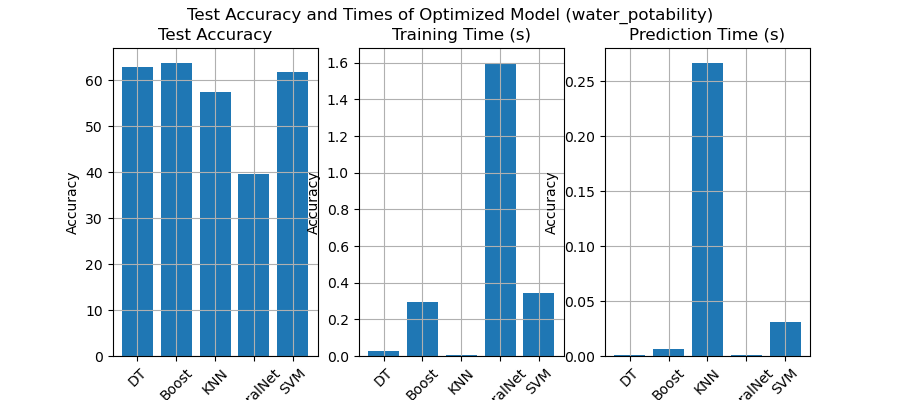
\includegraphics[width=0.90\textwidth]{../outputs/PerformanceComparison_water_potability.png}}}
	\caption{Performance comparison for the Water potability dataset. (left) Accuracy on test set (middle) Average training time (right) Average prediction time}
	\label{fig:fig1}
\end{figure}
\begin{figure}
	\centering
	{\frame{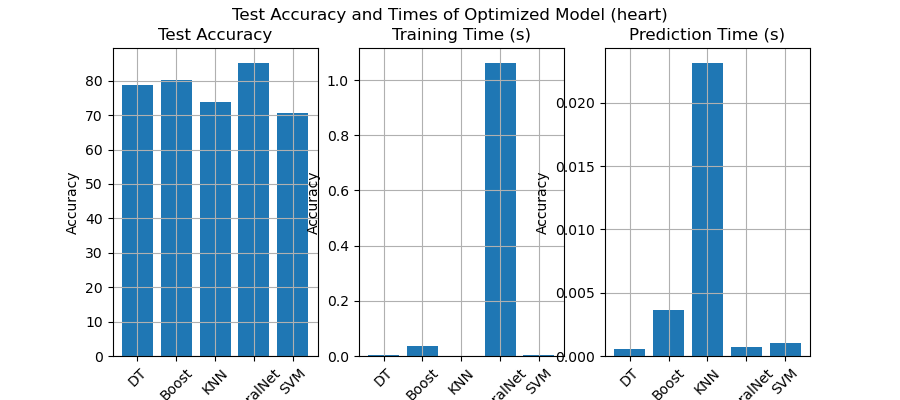
\includegraphics[width=0.90\textwidth]{../outputs/PerformanceComparison_heart.png}}}
	\caption{Performance comparison for the Heart dataset. (left) Accuracy on test set (middle) Average training time (right) Average prediction time}
	\label{fig:fig2}
\end{figure}

For figure 1 and figure 2, each model was tuned such that it acheived the highest cross-validation score, then predicted values for the test set. Both the cross-validation and test accuracy scores will be discussed further in each section, but this gives a good overview of the performance of each model.

\subsection{Decision Trees}
% TODO: Add runtimes to tables
A Decision Tree is a fairly simple model, but it turned out to be very effective. They are well suited for categorical classification, because of how they split data on different values within a feature. Integer or binned values tends to make it easier to split because the separation is more defined compared continuous values. So I expected DTs to perform well on both datasets, but not as well on the water data as the heart data. Because of the simplicity of decision trees, they are also the fastest model overall, with both training and predictions in the 2nd fastest of all models.
% accuracy table
\begin{center}
	\begin{tabular}{|c||c|c|c|c|}
	 \hline
	  & Cross Validation Score & Test Accuracy & Train Time & Predict Time \\
	 \hline\hline
	 Water Dataset & 63.5\%  & 62.8\% & 0.02988 & 0.0007560 \\
	 \hline
	 Heart Dataset & 78.5\%  & 78.7\% & 0.002586 & 0.0007398 \\
	 \hline
	\end{tabular}
	\label{table:table1}
\end{center}

% Decision Tree Plots - Water
\begin{figure}
	\centering
	\subfigure[]{\frame{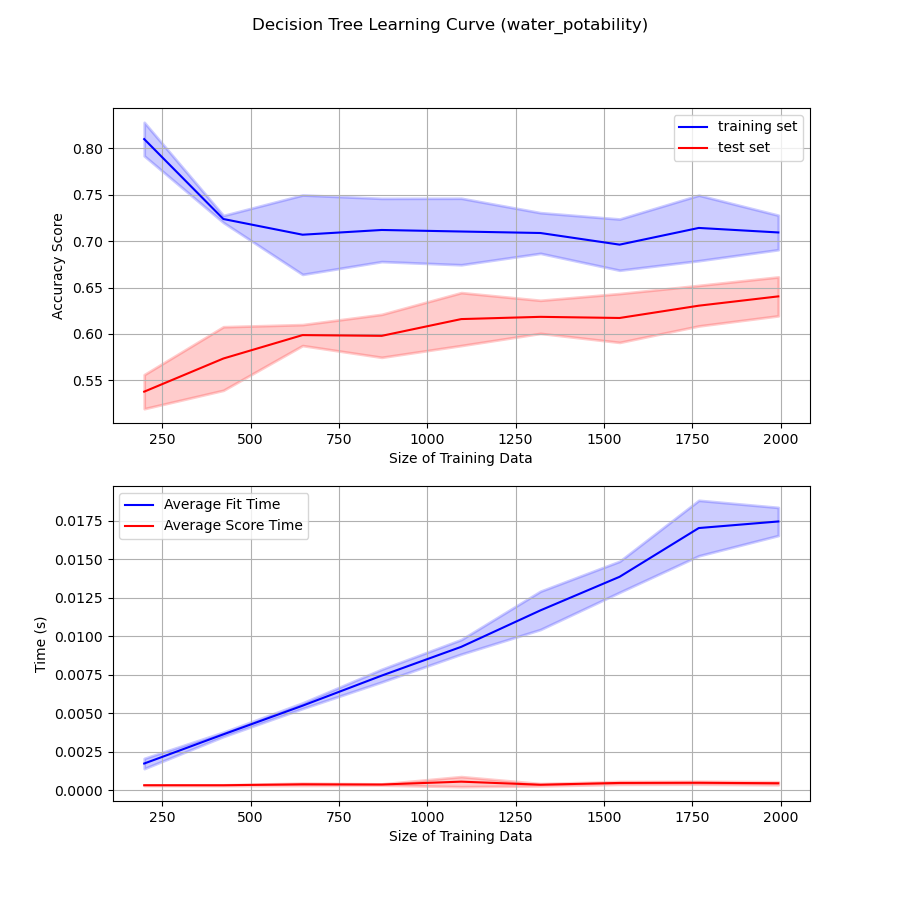
\includegraphics[width=0.40\textwidth]{../outputs/DT_LearningCurve_water_potability.png}}}
	\subfigure[]{\frame{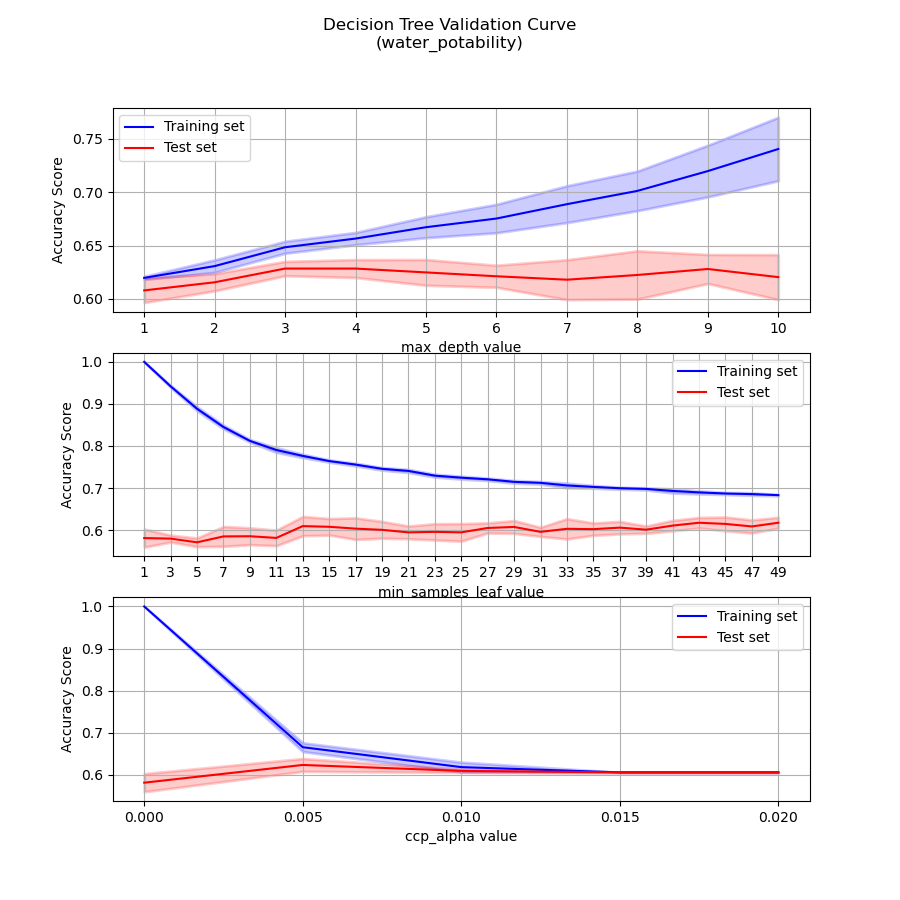
\includegraphics[width=0.40\textwidth]{../outputs/DT_ValidationCurve_water_potability.png}}}
	\caption{Decision Tree Model trained on the Water potability dataset. (a) Learning Curve and (b) Validation Curve}
	\label{fig:fig3}
\end{figure}
% Decision Tree Plots - Heart
\begin{figure}
	\centering
	\subfigure[]{\frame{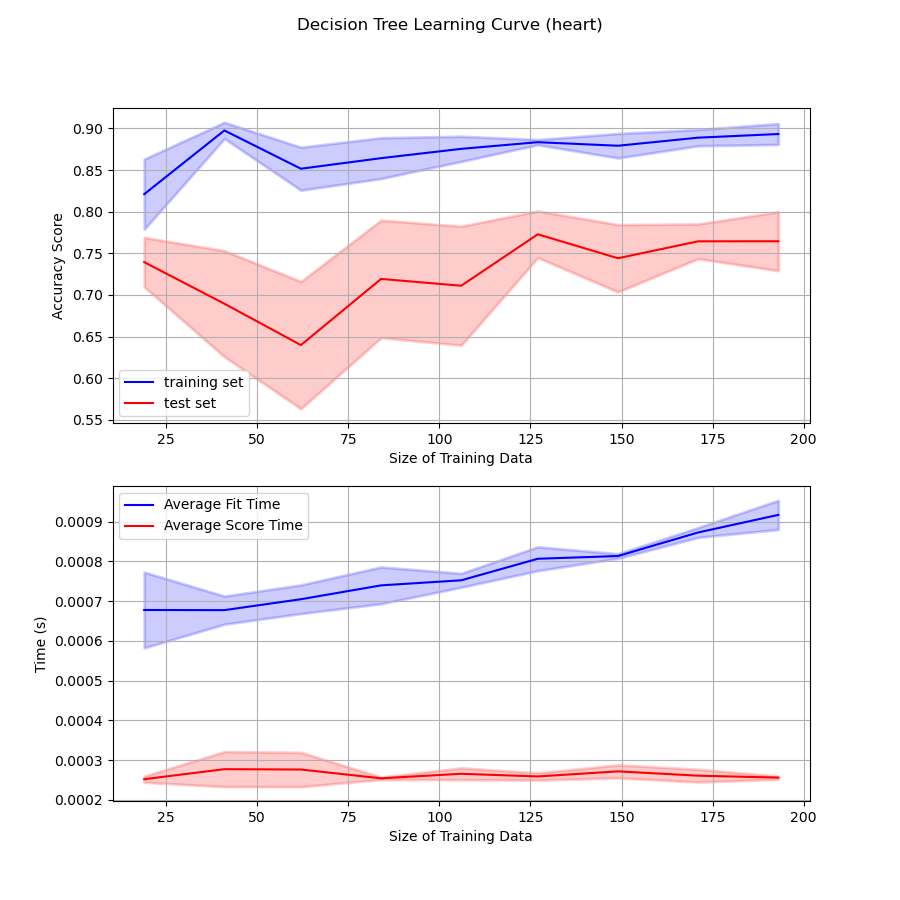
\includegraphics[width=0.40\textwidth]{../outputs/DT_LearningCurve_heart.png}}}
	\subfigure[]{\frame{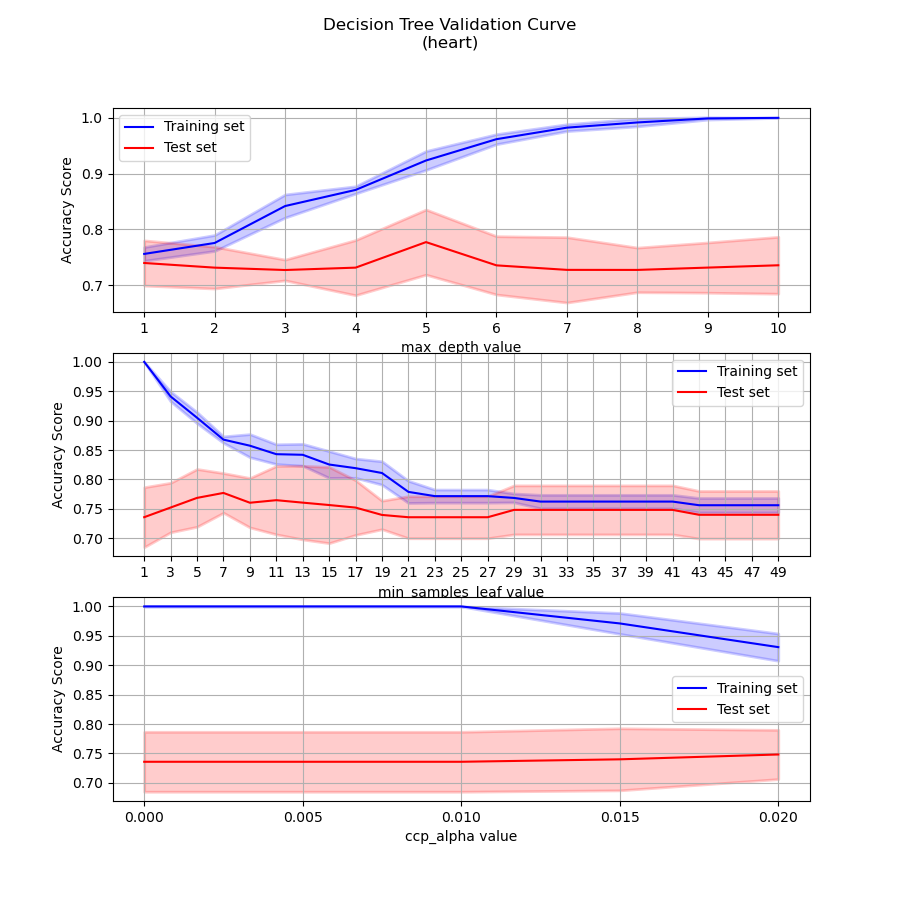
\includegraphics[width=0.40\textwidth]{../outputs/DT_ValidationCurve_heart.png}}}
	\caption{Decision Tree Model trained on the Heart dataset. (a) Learning Curve and (b) Validation Curve}
	\label{fig:fig4}
\end{figure}

In the learning curve, you can see clearly that for both datasets, the cross-validation accuracy increases as the training set increases. This means that both datasets are a little bit on the small side and could be improved by adding more data. Water potiblity is about 10 times the size of the heart dataset, but considering the fact that it has continuous features, it makes sense that it would be a little harder to classify. It is also important to note that the larger dataset, water potability, requires much more time to train, but the same amount of time to predict since there is more data that needed to go into the model, but in the end, traversing the tree is going to be roughly the same for each model.

The three parameters that I chose to optimize for DTs are max depth, min leaf size, and ccp alpha. Max depth limits how many splits down the tree can go before it must have a leaf node. Leaf size is similar in that it requires the tree to produce a leaf, but rather than constraining the depth of the tree, it constrains the size of the leaf. Each leaf must be no smaller than this parameter. Lastly is ccp alpha, which, from the sklearn docs, is a "Complexity parameter used for Minimal Cost-Complexity Pruning." It is a factor of post training pruning to reduce size and generalize better.

The reason I chose these three parameters are because they are the primary factors in determining how tightly the model fits to the data. They are all factors of pruning, although they each handle it in different ways. From the validation curves, you can see that max depth doesn't exactly have a direct correlation to accuracy, with both models peaking at different points. Similarly with leaf size, as the size increases, the training accuracy goes down, but the test accuracy slightly goes up, because it creates a more generalized model, rather than an overfitted model. The ccp alpha value causes a steep reduction in training accuracy, but a slight increase in test accuracy, although not much.

It should not be a surprise then that both both datasets, the optimal parameters were somewhere in the middle for max depth, relatively low for min leaf size, and low for ccp alpha, since the alpha value had a more significant effect on overall accuracy.

\subsection{AdaBoost}
AdaBoost is an ensamble learner, meaning it is a combination of multiple weak learners. In this implementation, it is a combination of a series of decision trees with high pruning. I used a somewhat arbitrary default decision tree so that I could focus my analysis on the Boosting model itself rather than the DT. For this reason, I kept the DT fixed with a max depth of 3, and varied the number of estimators and the learning rate. Boosting is a very useful model because it can take the strengths of a model such as decision trees, but by combining several of them together, it is able generalize better and reduces the amount of overfitting. This comes at a cost of speed. Since there are multiple decision trees being trained and used for prediction, it makes them much slower than decision trees, although still faster than some others.

% accuracy table
\begin{center}
	\begin{tabular}{|c||c|c|c|c|}
	 \hline
	  & Cross Validation Score & Test Accuracy & Train Time & Predict Time \\
	 \hline\hline
	 Water Dataset & 64.1\%  & 63.8\% & 0.2863 & 0.0066242 \\
	 \hline
	 Heart Dataset & 80.2\%  & 80.3\% & 0.03972 & 0.004307\\
	 \hline
	\end{tabular}
	\label{table:table2}
\end{center}
% Boost plots - Water
\begin{figure}
	\centering
	\subfigure[]{\frame{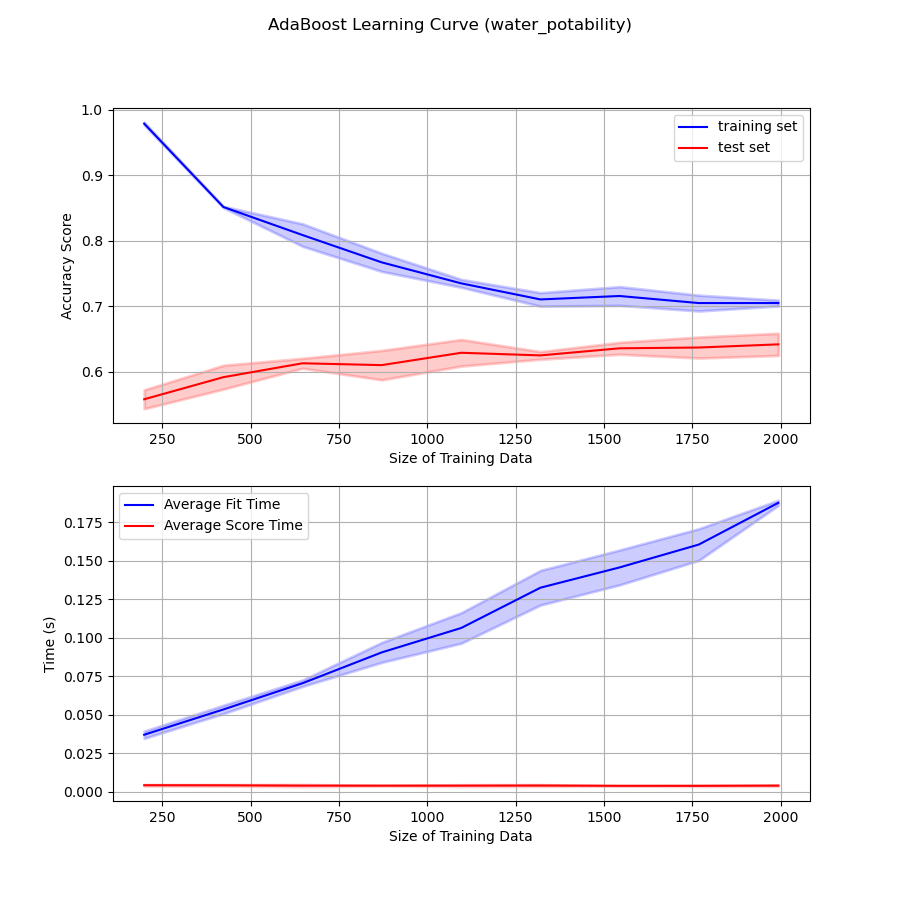
\includegraphics[width=0.40\textwidth]{../outputs/Boost_LearningCurve_water_potability.png}}}
	\subfigure[]{\frame{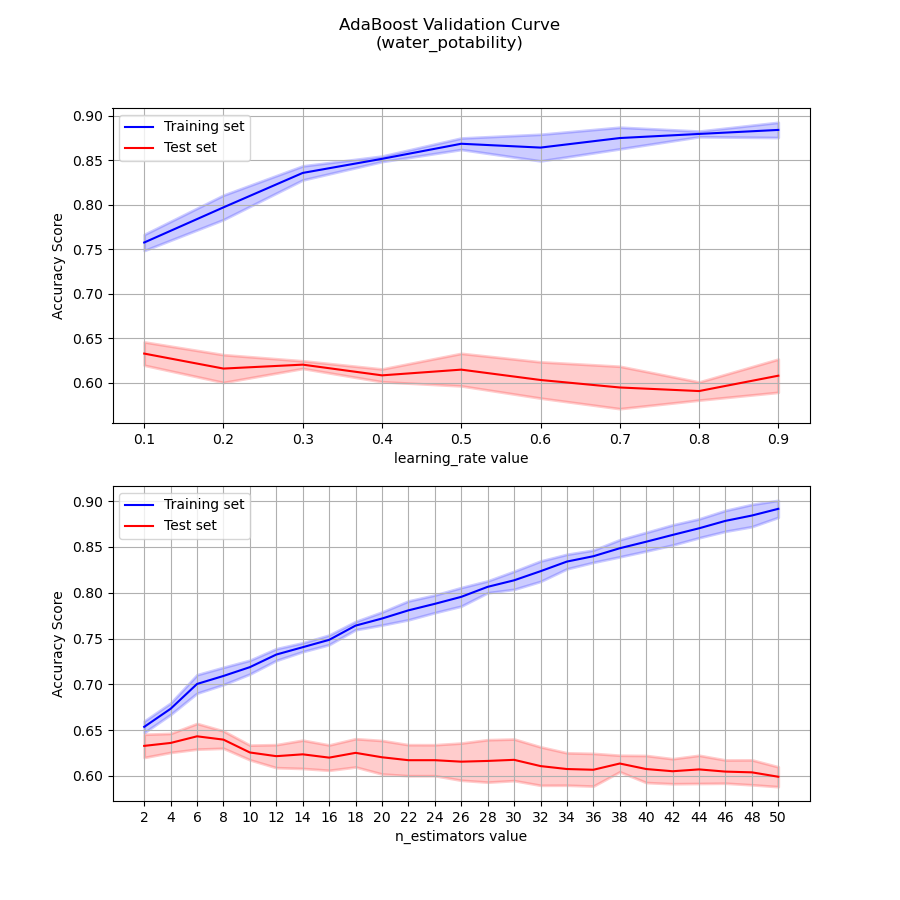
\includegraphics[width=0.40\textwidth]{../outputs/Boost_ValidationCurve_water_potability.png}}}
	\caption{AdaBoost Model trained on water potability dataset. (a) Learning Curve and (b) Validation Curve}
	\label{fig:fig5}
\end{figure}
% Boost plots - Heart
\begin{figure}
	\centering
	\subfigure[]{\frame{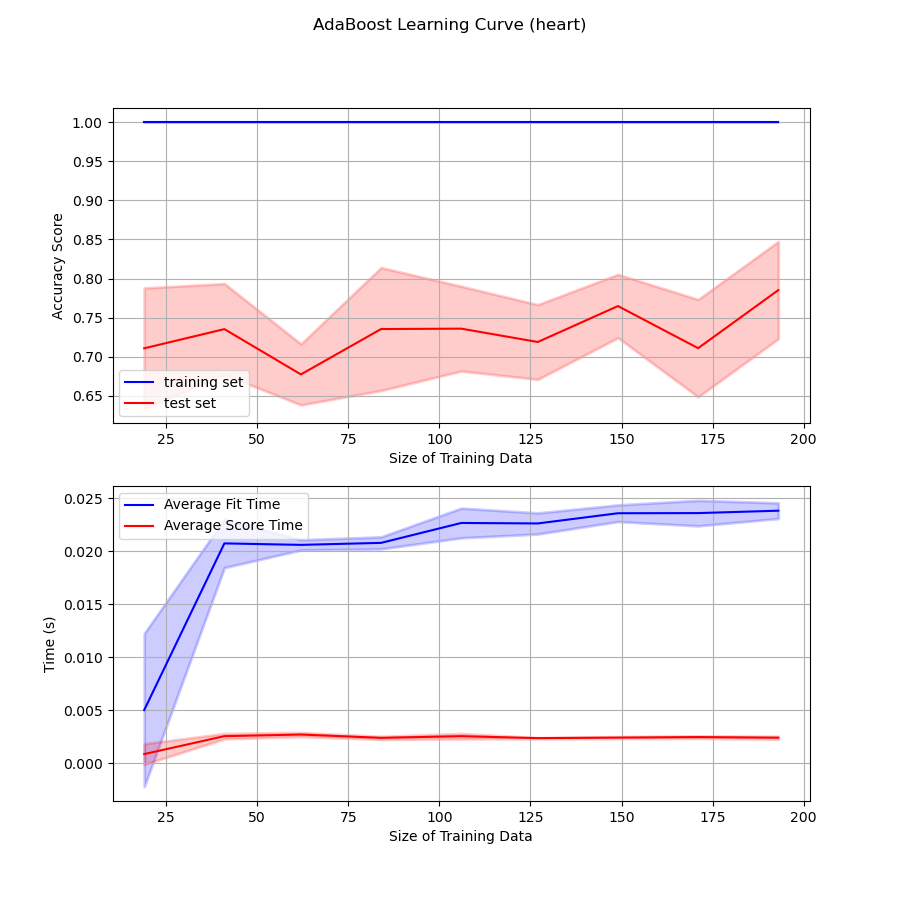
\includegraphics[width=0.40\textwidth]{../outputs/Boost_LearningCurve_heart.png}}}
	\subfigure[]{\frame{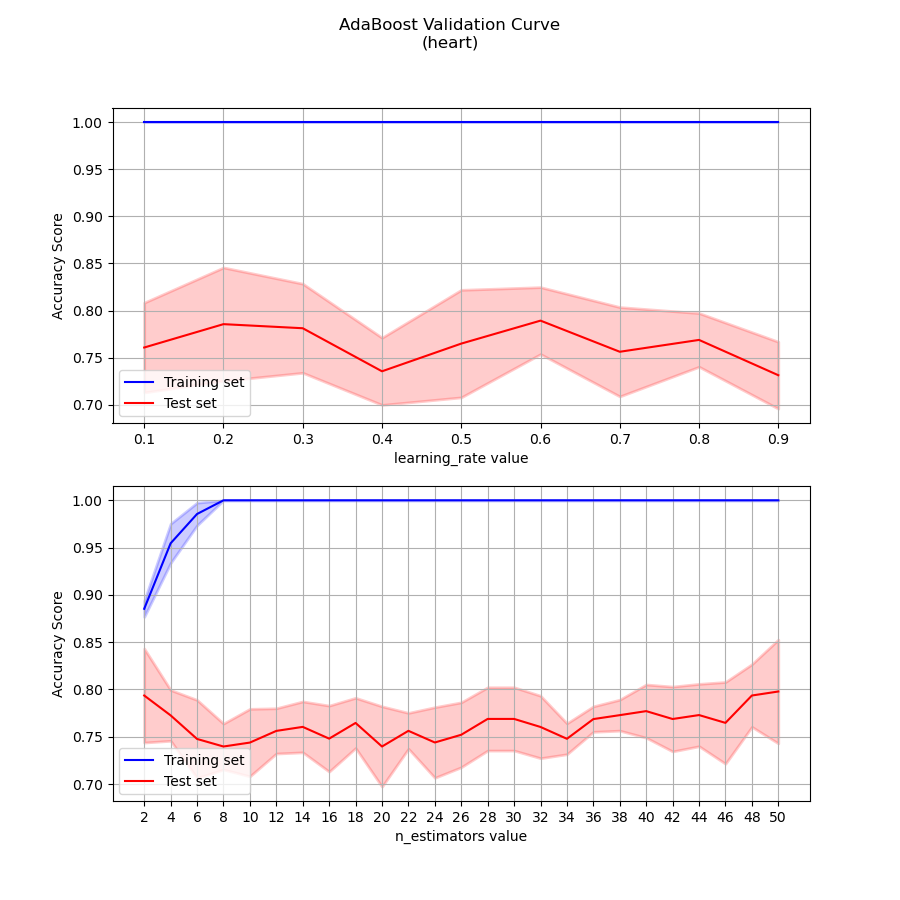
\includegraphics[width=0.40\textwidth]{../outputs/Boost_ValidationCurve_heart.png}}}
	\caption{AdaBoost Model trained on heart dataset. (a) Learning Curve and (b) Validation Curve}
	\label{fig:fig6}
\end{figure}

AdaBoost performed just slightly better than decision trees on both datasets, and had the best generalized representation of all 5 models tested. Both the training and test accuracy was less than 0.5\% different between the two. Just as with decision trees, the learning curve shows that the higher the amount of training data, the better the performance. This means that either the datasets are too small, or that both DT and Boosting require a lot of data to perform well.

The two main parameters when designing a Boosting model are the number of estimators, and the learning rate. The number of estimators is obviously the number of instances of the DT model, and the learning rate is the weight applied to each iteration. It primarily affects how quickly the model learns, although can have an affect on accuracy as well. ALthough not plotted here, higher learning rate makes the model converge more quickly, but as you can see in the validation curve, it also tends to be less accurate. One would expect that higher values for estimators, and lower values of learning rate would be optimal. In both datasets, the models converged at estimators in the low 20s and learning rates at 0.5 or less.

\subsection{Neural Networks}
Neural Networks turned out to be one of the most interesting models I worked with. Because of their ability to catch complexity in data, I expected them to be the highest performing for the water potability dataset, but I encountered some unexpected results. Training is very math intense, so I was not at all surprised to see that they had the slowest training of all models by far. This can very a lot depending on the complexity of the network, but exen relatively simple networks can take a while to train. However, once they are trained, the predictions are just about as fast as decision trees.

% accuracy table
\begin{center}
	\begin{tabular}{|c||c|c|c|c|}
	 \hline
	  & Cross Validation Score & Test Accuracy & Train Time & Predict Time \\
	 \hline\hline
	 Water Dataset & 67.9\%  & 39.6\% & 1.785 & 0.001204 \\
	 \hline
	 Heart Dataset & 83.9\%  & 73.8\% & 1.174 & 0.001129 \\
	 \hline
	\end{tabular}
	\label{table:table3}
\end{center}
% Neural Net Plots - Water
\begin{figure}
	\centering
	\subfigure[]{\frame{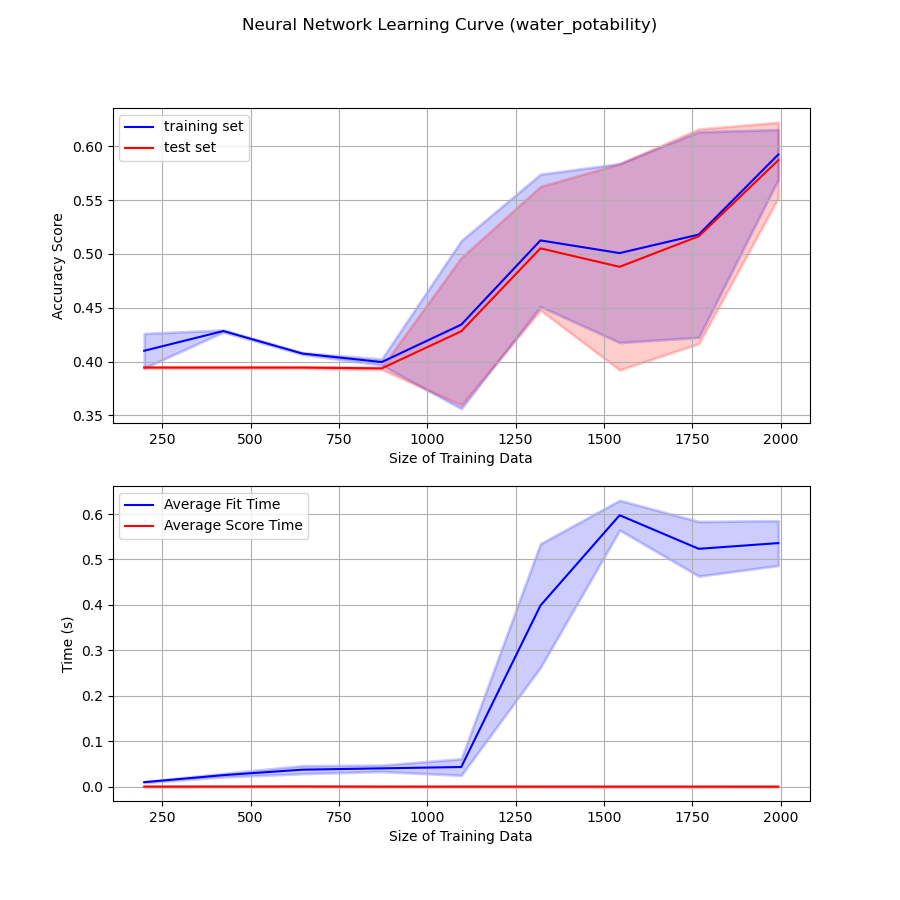
\includegraphics[width=0.40\textwidth]{../outputs/NN_LearningCurve_water_potability.png}}}
	\subfigure[]{\frame{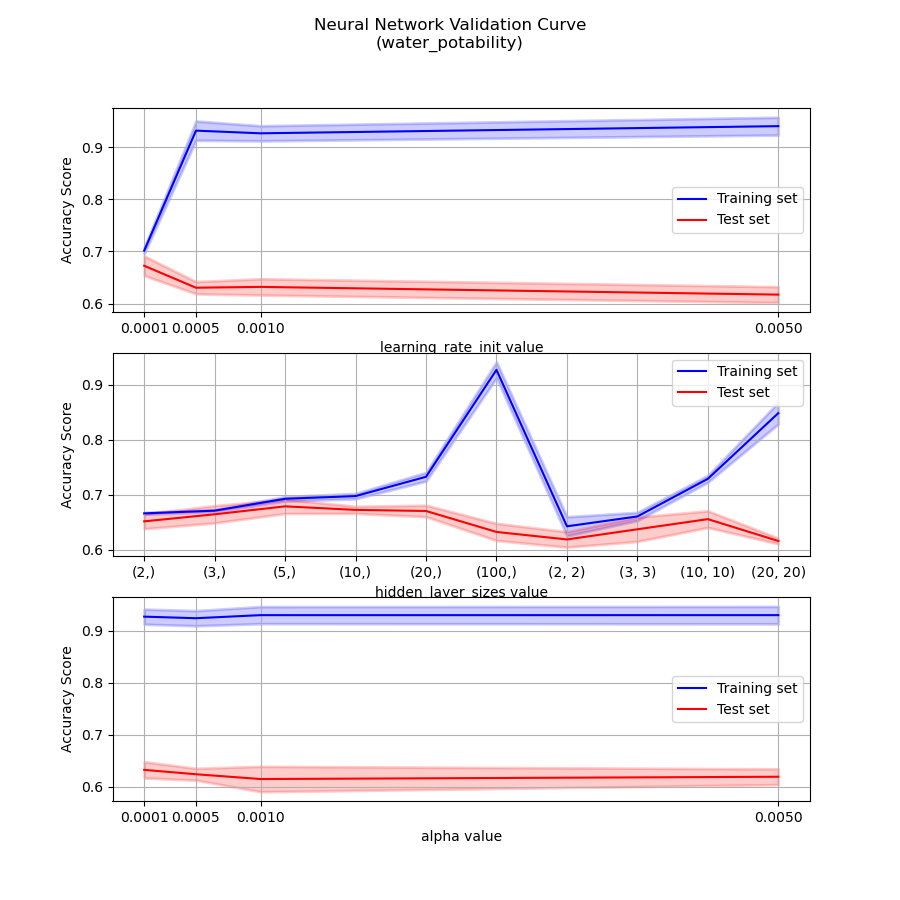
\includegraphics[width=0.40\textwidth]{../outputs/NN_ValidationCurve_water_potability.png}}}
	\caption{Neural Network Model trained on water potability dataset (a) Learning Curve and (b) Validation Curve}
	\label{fig:fig7}
\end{figure}
% Neural Net Plots - heart
\begin{figure}
	\centering
	\subfigure[]{\frame{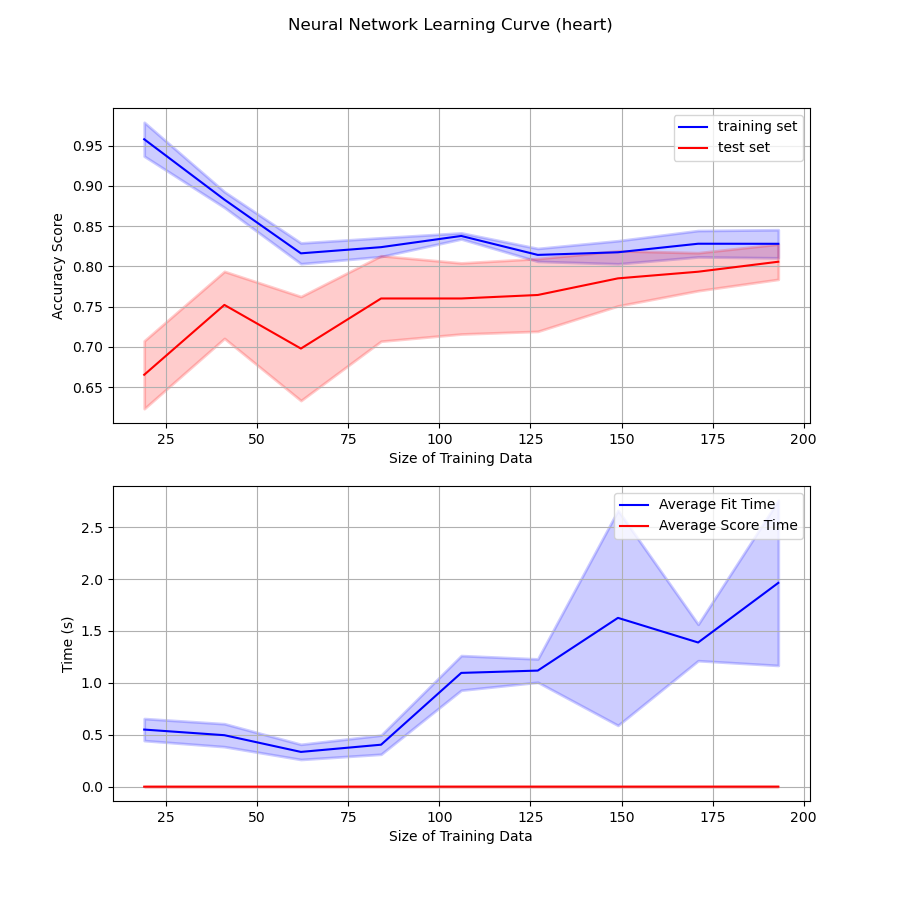
\includegraphics[width=0.40\textwidth]{../outputs/NN_LearningCurve_heart.png}}}
	\subfigure[]{\frame{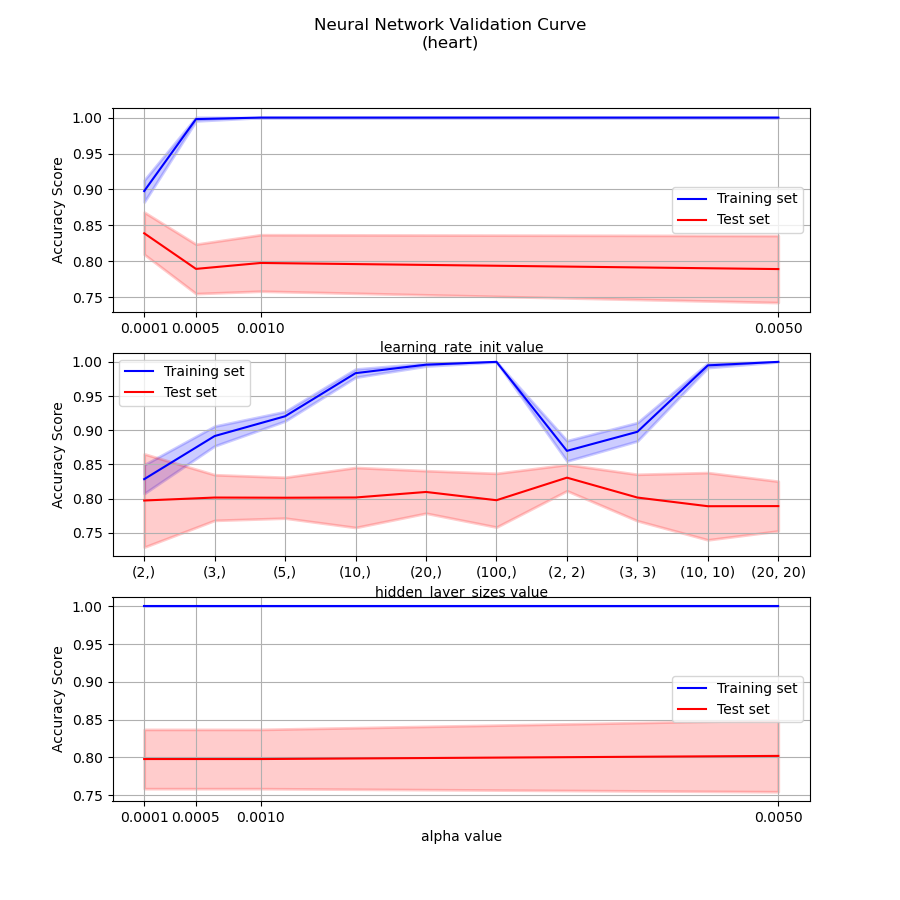
\includegraphics[width=0.40\textwidth]{../outputs/NN_ValidationCurve_heart.png}}}
	\caption{Neural Network Model trained on heart dataset (a) Learning Curve and (b) Validation Curve}
	\label{fig:fig8}
\end{figure}
% Neural Net Plots - Loss
\begin{figure}
	\centering
	\subfigure[]{\frame{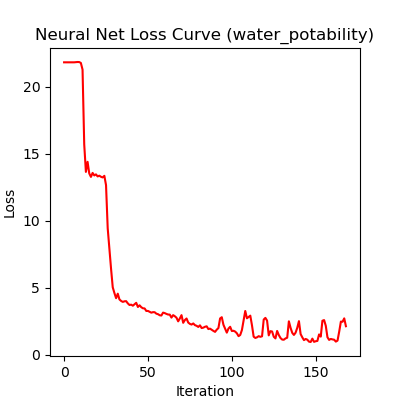
\includegraphics[width=0.40\textwidth]{../outputs/NN_LossGraph_water_potability.png}}}
	\subfigure[]{\frame{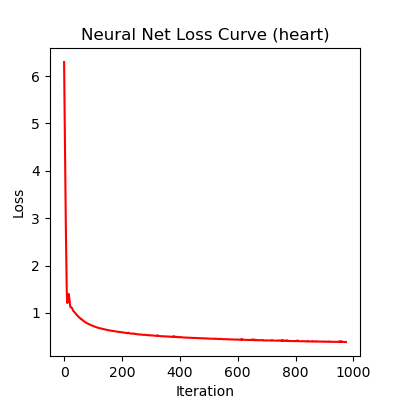
\includegraphics[width=0.40\textwidth]{../outputs/NN_LossGraph_heart.png}}}
	\caption{Neural Network Loss graph for: (a) water potability dataset and (b) heart dataset}
	\label{fig:fig9}
\end{figure}

The first thing to notice with the results is that there is clearly something wrong with how the neural network handled the water data. After much trial and error, I was not able to figure out what the issue was, and settled on the best that I could get. It seems like there is possibly either something wrong with how I handled the data pre-processing, or the complexity of the model meant that it was not linearly separable, resulting in sub-optimal results. Either way, it is interesting that the water dataset performed so well on other models, and even in cross validation on neural networks, but failed on test accuracy.

Neural Networks, just like decision trees, need a lot of data to get valuable results. On both datasets, the accuracy improves with more data, and also increases the training time, but does not affect the prediction time. This is no surprise, because more data means more number crunching to optimize the weights, but it doesn't change the forward pass at all when it comes to prediction. The equation will be the same, just with different values, regardless of the input data.

While there are many different parameters that can be tuned on neural networks, I want to keep it relatively simple and focus on the more outwardly changing ones. What I mean by that is the parameters that have a more visible change to the model rather than just some of the math that is happening under the hood. For this reason I chose the learning rate, hidden layers, and alpha value. The learning rate is similar to AdaBoost, and lower learning rate leads to sometimes more optimal models, but slower training times. I chose a range of layers to test out, from very small single hidden layers to much larger double layers, to see how they would affect the performance. More nodes means higher capability to learn details of the model, but that also means higher change of overfitting.

The validation curves seem to match what I expected. essentially, the higher number of nodes, the higher the overfitting, so the optimal should be at some middle value. However, in the water set, my model determined that a single layer of 10 nodes was the best, and in the heart dataset the model determined that a single layer of 100 nodes was best. Neither of these seem to match the validation curves which show (5,) and (10, 10) as the optimal for water, and (2, 2) as the optimal for the heart dataset. There seemed to be a strange combination of factors on the water dataset that lead to a very strong cross validation score that just didn't translate over to the test data. You can also see from the loss curve for the water data that there was not a smooth reduction in loss like there was for the heart data.

The alpha term is the regularization parameter, which did not seem to have a strong affect on the results at all.

\subsection{Support Vector Machines}
Support Vector Machines work by attempting to segment data into classes using hyperplanes. It is somewhat similar to KNN (which will be covered next) in that it uses how values compare to others in the set to determine the best way to segment the data. It is well suited for smaller datasets because it can gain a lot of information with less points. Larger datasets also greatly increase both the training time and prediction time, as you can see the difference between the water set, which has around 2000 data points, and the heart set, which has around 200.

% accuracy table
\begin{center}
	\begin{tabular}{|c||c|c|c|c|}
	 \hline
	  & Cross Validation Score & Test Accuracy & Train Time & Predict Time \\
	 \hline\hline
	 Water Dataset & 67.3\%  & 61.8\% & 0.3396 & 0.0295 \\
	 \hline
	 Heart Dataset & 84.7\%  & 70.5\% & 0.003217 & 0.0008929\\
	 \hline
	\end{tabular}
	\label{table:table4}
\end{center}
% SVM Plots - water
\begin{figure}
	\centering
	\subfigure[]{\frame{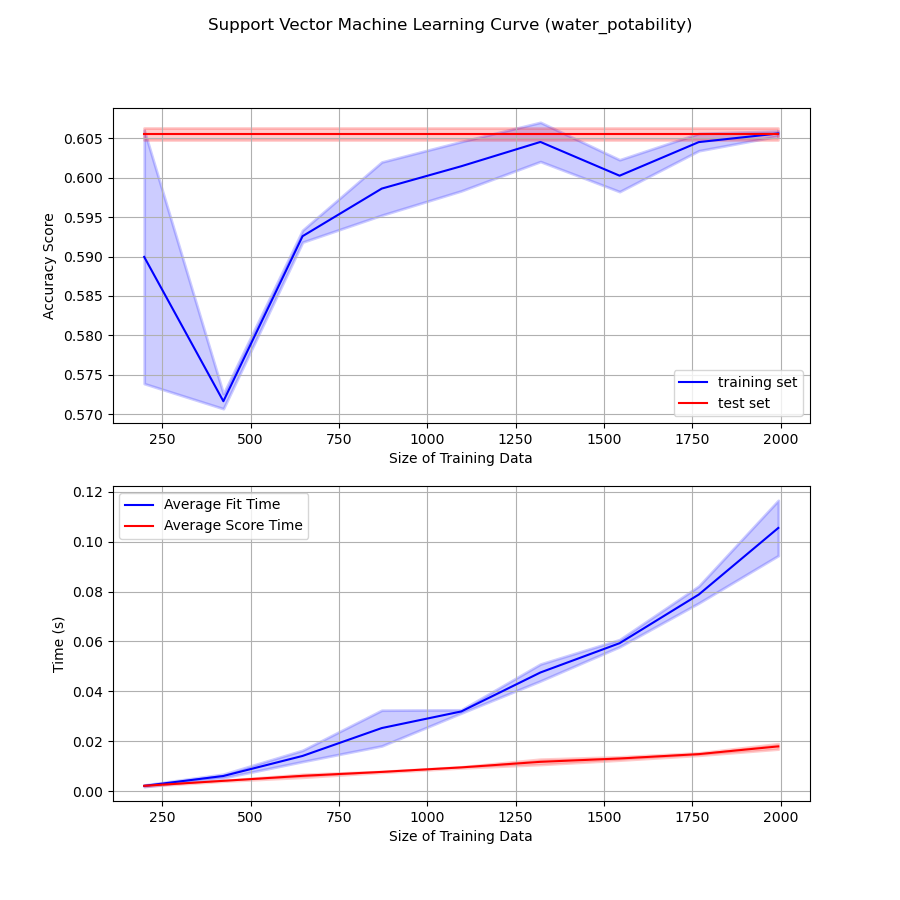
\includegraphics[width=0.40\textwidth]{../outputs/SVM_LearningCurve_water_potability.png}}}
	\subfigure[]{\frame{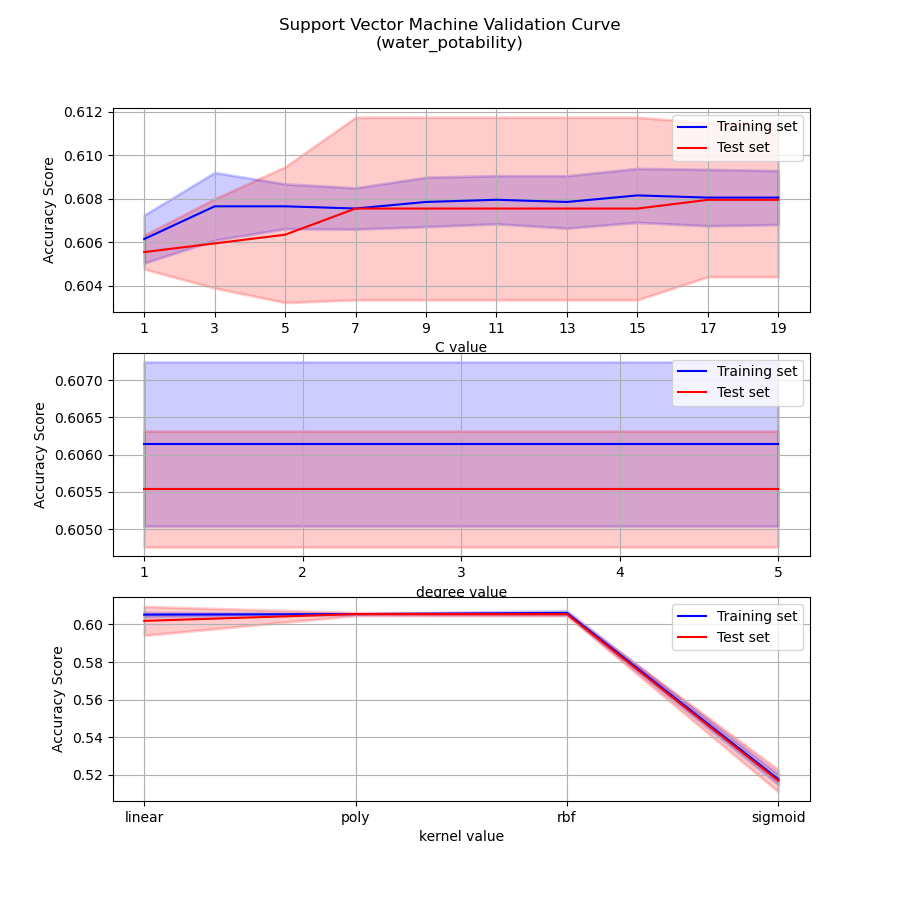
\includegraphics[width=0.40\textwidth]{../outputs/SVM_ValidationCurve_water_potability.png}}}
	\caption{SVM Model trained on water potability dataset. (a) Learning Curve and (b) Validation Curve}
	\label{fig:fig10}
\end{figure}
% SVM Plots - heart
\begin{figure}
	\centering
	\subfigure[]{\frame{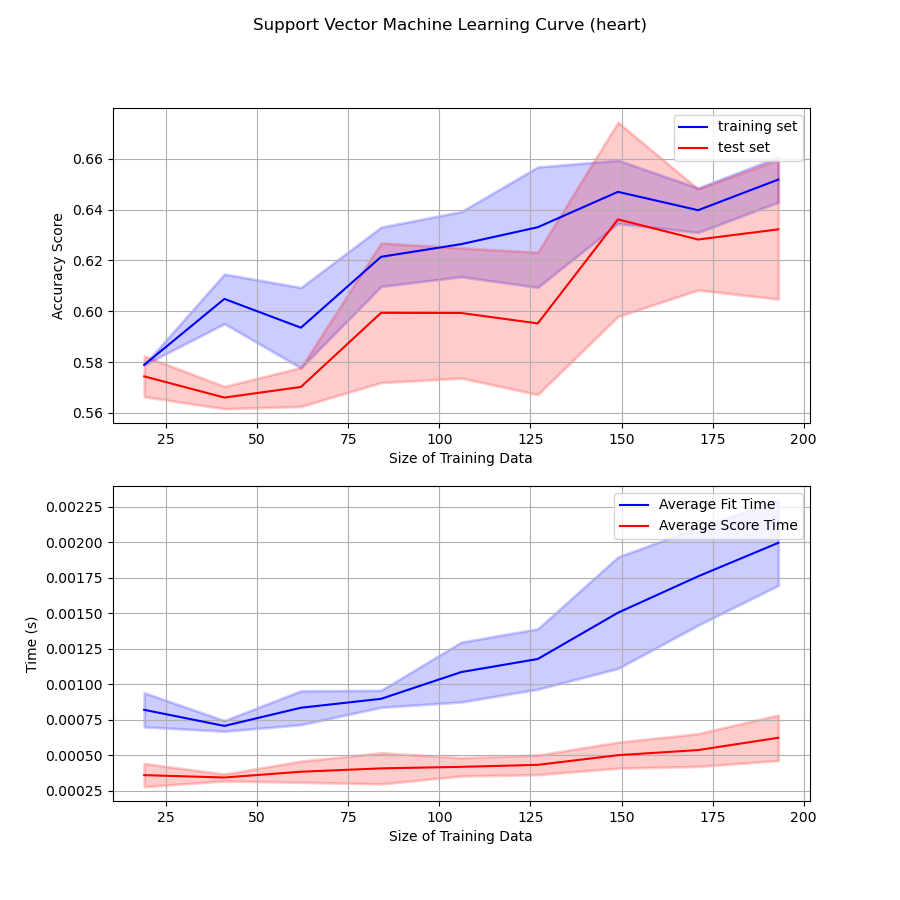
\includegraphics[width=0.40\textwidth]{../outputs/SVM_LearningCurve_heart.png}}}
	\subfigure[]{\frame{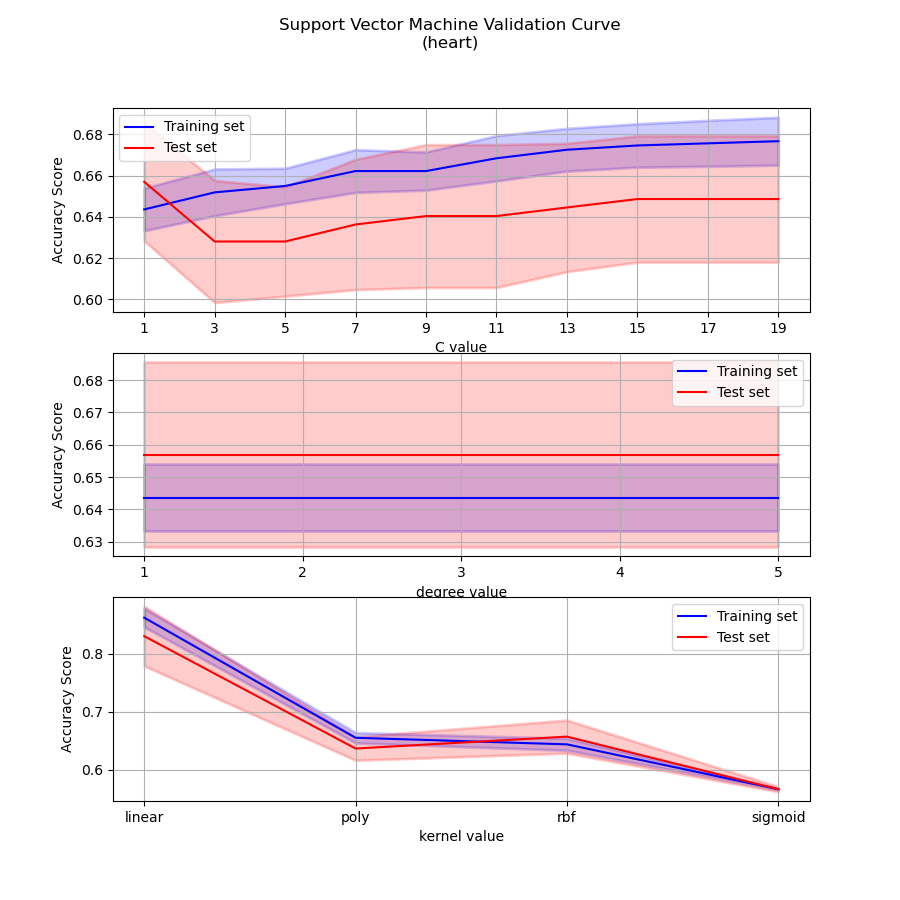
\includegraphics[width=0.40\textwidth]{../outputs/SVM_ValidationCurve_heart.png}}}
	\caption{SVM Model trained on heart dataset. (a) Learning Curve and (b) Validation Curve}
	\label{fig:fig11}
\end{figure}

Similar to the Neural Networks, I experienced some unexpected results, which are likely caused by some error in data processing. However, the training and prediction times are very clear. The prediction time has a mostly linear increase in time with larger datasets, while the training time is exponential.

The main parameters for a SVM model are the kernel, which is basically the kind of formula used to generate the hyperplane, the degree (which only applied to a polynomial kernal), and the C value. The C parameter is a regularization parameter. Higher C values mean a smaller margin hyperplane with less misclassified points, where a lower C value has a larger margin, though may have more misclassifications. A C value too high could result in overfitting.

The type of kernel depends on the data. As you can see clearly, the heart data performs very will with a linear kernel, and much lower results on any of the others, while the water data performs relatively well on all but sigmoid. I don't know why exactly the sigmoid performs poorly, but considering that the water data is all continuous, it makes sense that more complex kernels perform better, such as the rbf and polynomial, where the linear performs well on the heart data, which is mostly categorical.

\subsection{K-Nearest Neighbor}
K Nearest Neighbor is another simple but effective model for classification. The primary advantage of KNN is that it requires almost no training. There are some steps that can be taken during training to optimize the search for nearest neighbors, but there isn't any true training taking place, since all the work is done during prediction time. This is why for both datasets, KNN had the fastest training time, and the slowest prediction time. It's also worth noting just how much slower it was in the water dataset, which is about 10 times the size of the heart dataset.

% accuracy table
\begin{center}
	\begin{tabular}{|c||c|c|c|c|}
	 \hline
	  & Cross Validation Score & Test Accuracy & Train Time & Predict Time \\
	 \hline\hline
	 Water Dataset & 64.8\%  & 57.4\% & 0.003573 & 0.2185 \\
	 \hline
	 Heart Dataset & 84.7\%  & 73.8\% & 0.002100 & 0.01965\\
	 \hline
	\end{tabular}
	\label{table:table5}
\end{center}
% KNN Plots - water
\begin{figure}
	\centering
	\subfigure[]{\frame{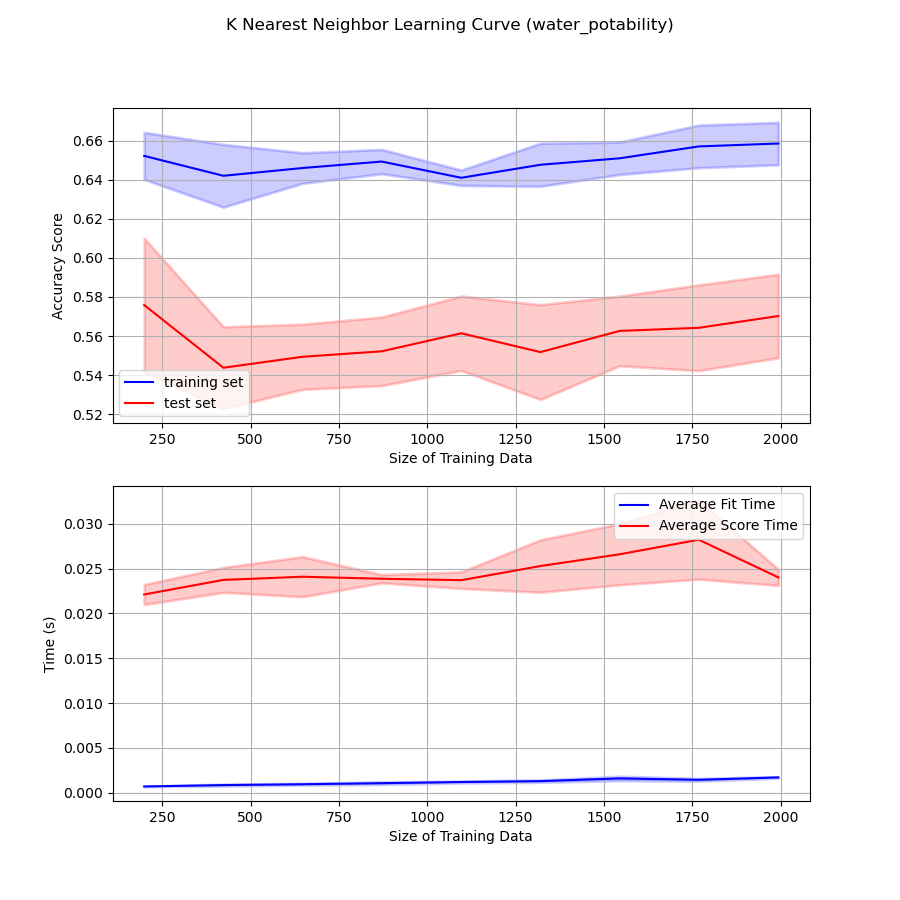
\includegraphics[width=0.40\textwidth]{../outputs/KNN_LearningCurve_water_potability.png}}}
	\subfigure[]{\frame{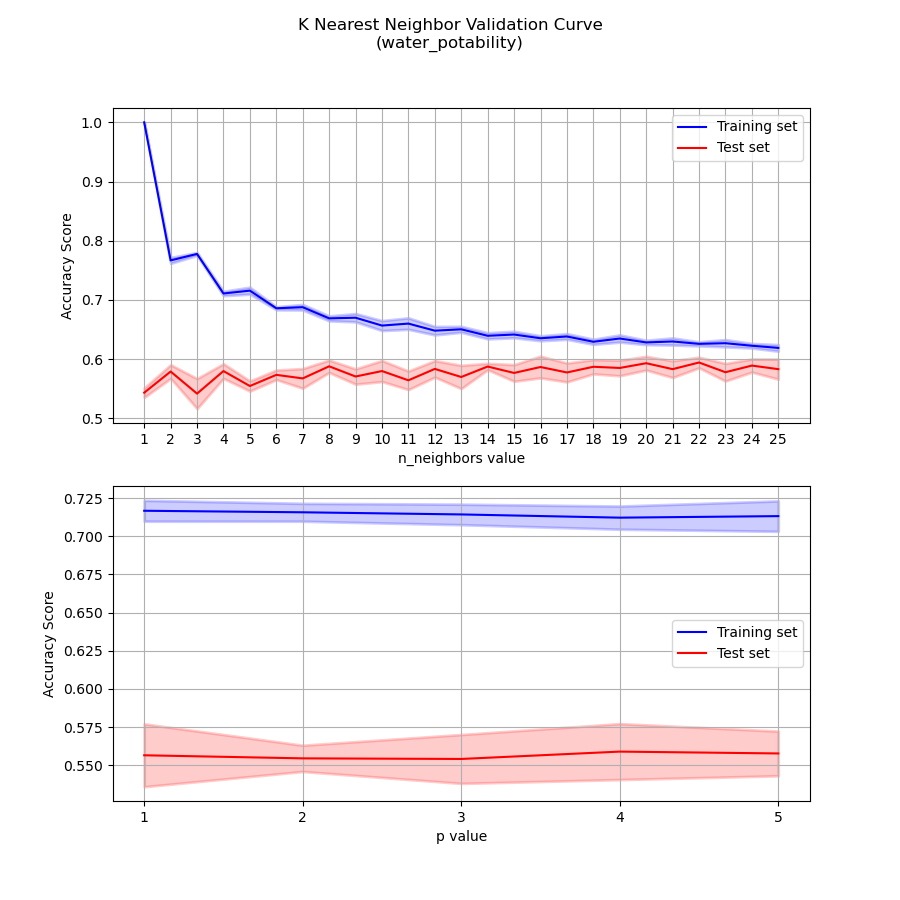
\includegraphics[width=0.40\textwidth]{../outputs/KNN_ValidationCurve_water_potability.png}}}
	\caption{KNN Model trained on water potability dataset. (a) Learning Curve and (b) Validation Curve}
	\label{fig:fig12}
\end{figure}
% KNN Plots - water
\begin{figure}
	\centering
	\subfigure[]{\frame{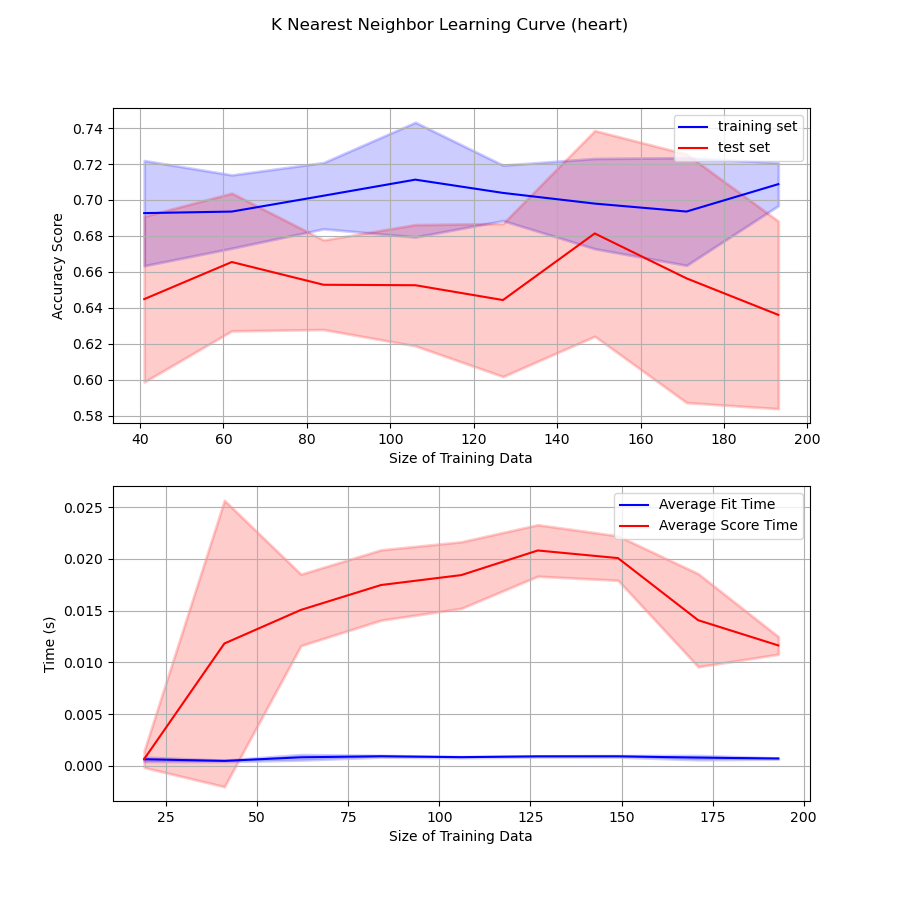
\includegraphics[width=0.40\textwidth]{../outputs/KNN_LearningCurve_heart.png}}}
	\subfigure[]{\frame{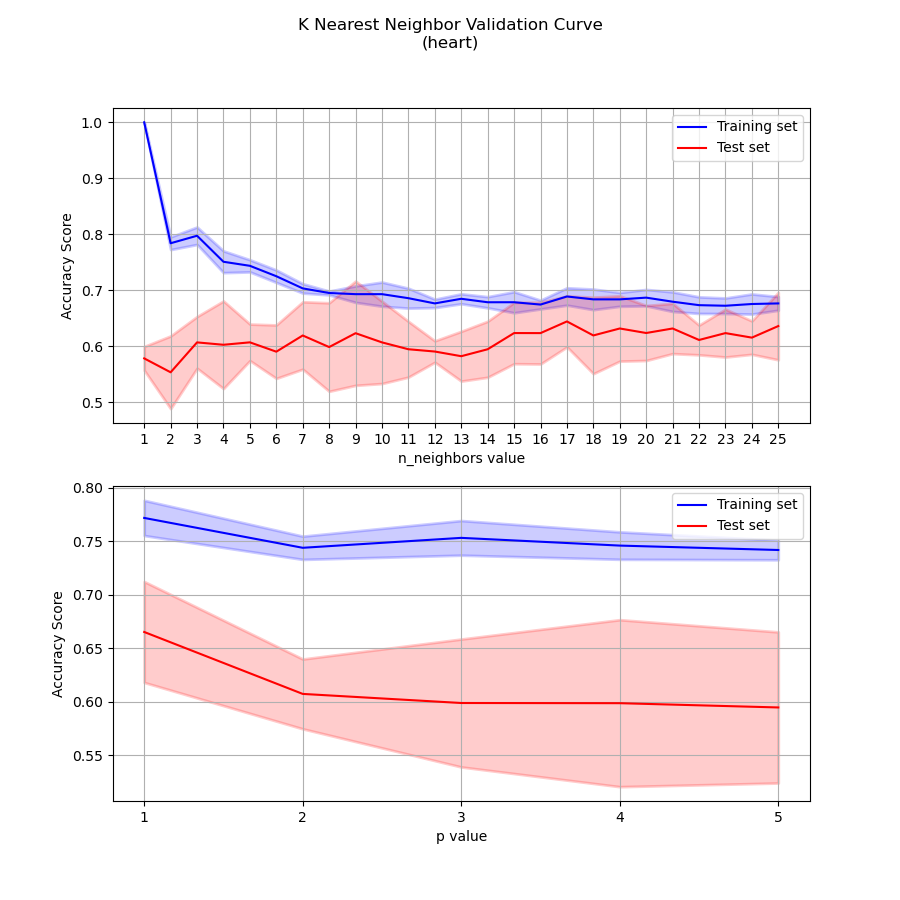
\includegraphics[width=0.40\textwidth]{../outputs/KNN_ValidationCurve_heart.png}}}
	\caption{KNN Model trained on heart dataset. (a) Learning Curve and (b) Validation Curve}
	\label{fig:fig13}
\end{figure}

The main parameters for KNN are the K value (number of neighbors) and the parameter, p, which is a power factor which affects how much distance plays into the association. Higher values of p put greater weight on points closer to the prediction point. Surprisingly, the p factor had little affect on either dataset, with almost no noticeable affect at all on the water data. Given that it is continuous data, it does make sense that it would be more challenging to classify, but it is surprising that accuracy actually decreases with high p value in the heart data. One would think that closer points should be given a much higher weight, but apparently that was not the case for these datasets.

The largest factor was in the number of neighbors. Low K values means greater overfitting, and higher values means more generalization. It would stand to reason that the optimal value should be somewhere in the middle. In this sense KNN is fairly predictable, but the exact values changed based on the model. Water only needed 11 neighbors, while the heart data needed 22.

\section{Conclusion}
While there is not a significant difference in the style of data between the two datasets I chose, there were some interesting differences. The two main differences between these datasets are the size (roughly 3000 points compared to roughly 300) and the type of data (continuous vs categorical). Even though the Water potability data is a binary classifier, each model still had a hard time getting high levels of accuracy, although still manage to perform consistently better than guessing. The only exception was the Neural Network, which likely had some errors in pre-processing.

The models highlighted some valuable tradeoffs when it comes to their performance. Neural Networks, while producing the highest accuracy, take a significant amount of time to train, and therefore, may not be the right choice if there is a lot of data or if it needs to be set up quickly. It also is apparently sensitive to pre-processing. KNN is the opposite. while it generally did not perform quite as well as the other models in accuracy, it was the fastest to setup. Decision Trees and Boosting proved to be a very solid middle ground, with relatively high accuracy, and surprisingly low overfitting or underfitting if pruned right. Boosting in particular was almost perfect when it came to making a generalized model, and while a bit slower than most others in both training and predicting, still was not bad compared to the worst models. Boosting also proved to be very flexible in that it worked well for both continuous and categorical data.

If there was anythign I could do differently, it would be to spend more time in getting the data processed correctly. I think this would have made a very noticeable difference in the Neural Networks and SVM, but could have potentially played into the other models as well.

\newpage

\section{References}
\nocite{water}
\nocite{heart}
\nocite{Mitchell}
\printbibliography

\end{document}